\pagebreak
\section*{Tydzień 3}
Dyskretne systemy dynamiczne
%###################                 3.1.1              #################################%
\subsection*{Zadanie 3.1.1} {\color{darkgray}
	Narysować rozwiązanie równania różnicowego $x(k+1)=\lambda_ix(k)$\\
	 dla $i=1,2,3$ gdzie \\
	$\lambda_1 = 0, \lambda_2=1, \lambda_3=-1$ \\
	przy czym $x(0)=-1$ i $k\geq0$
}\\\\
\noindent$\bullet\ \ i=3, \lambda_i = -1$\\
$x(k)=(-1)^k(-1)=(-1)^{k+1}$

\begin{figure}[!h]
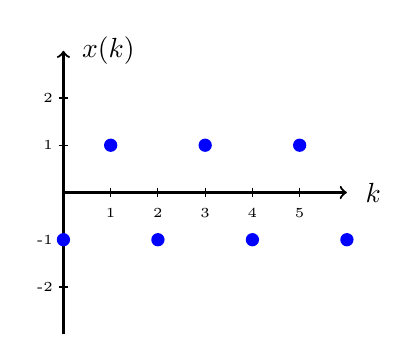
\begin{tikzpicture}[scale=0.6]
	\draw[thick][->](0,0)--(6,0) node [right=3pt]{$k$};
	\draw[thick][->](0,-3)--(0,3) node [right=3pt]{$x(k)$};

	\foreach \y [count=\i] in {-2,...,-1} {{
	     \draw (-0.1,\y) -- (0.1,\y) node [left=2pt]{{\tiny \y}};
 	}}
	\foreach \y [count=\i] in {1,...,2} {{
	     \draw (-0.1,\y) -- (0.1,\y) node [left=2pt]{{\tiny \y}};
 	}}
	\foreach \x [count=\i] in {-4,...,-1} {{
	    % \draw (\x,-0.1) -- (\x,0.1) node [below=4pt]{{\tiny \x}};
 	}}
	\foreach \x [count=\i] in {1,...,5} {{
	     \draw (\x,-0.1) -- (\x,0.1) node [below=4pt]{{\tiny \x}};
 	}}
		
	% koniec Osi
	
	\fill[fill=blue](0,-1) circle(4pt);
	\fill[fill=blue](1,1) circle(4pt);
	\fill[fill=blue](2,-1) circle(4pt);
	\fill[fill=blue](3,1) circle(4pt);
	\fill[fill=blue](4,-1) circle(4pt);
	\fill[fill=blue](5,1) circle(4pt);
	\fill[fill=blue](6,-1) circle(4pt);
\end{tikzpicture}
\end{figure}


\noindent$\bullet\ \ i=2, \lambda_i = 1$\\
$x(k)=(1)^k(-1)=-1$

\begin{figure}[!h]
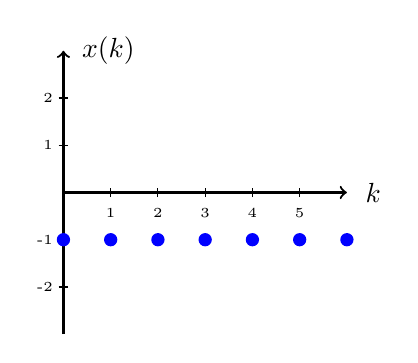
\begin{tikzpicture}[scale=0.6]
	\draw[thick][->](0,0)--(6,0) node [right=3pt]{$k$};
	\draw[thick][->](0,-3)--(0,3) node [right=3pt]{$x(k)$};

	\foreach \y [count=\i] in {-2,...,-1} {{
	     \draw (-0.1,\y) -- (0.1,\y) node [left=2pt]{{\tiny \y}};
 	}}
	\foreach \y [count=\i] in {1,...,2} {{
	     \draw (-0.1,\y) -- (0.1,\y) node [left=2pt]{{\tiny \y}};
 	}}
	\foreach \x [count=\i] in {-4,...,-1} {{
	    % \draw (\x,-0.1) -- (\x,0.1) node [below=4pt]{{\tiny \x}};
 	}}
	\foreach \x [count=\i] in {1,...,5} {{
	     \draw (\x,-0.1) -- (\x,0.1) node [below=4pt]{{\tiny \x}};
 	}}
		
	% koniec Osi
	
	\fill[fill=blue](0,-1) circle(4pt);
	\fill[fill=blue](1,-1) circle(4pt);
	\fill[fill=blue](2,-1) circle(4pt);
	\fill[fill=blue](3,-1) circle(4pt);
	\fill[fill=blue](4,-1) circle(4pt);
	\fill[fill=blue](5,-1) circle(4pt);
	\fill[fill=blue](6,-1) circle(4pt);
\end{tikzpicture}
\end{figure}

\noindent$\bullet\ \ i=0, \lambda_i = 0$\\
$x(k)=(0)^k(-1)=
	\begin{cases}
   	-1 &\text{dla } k=0\\
	0  &\text{dla } k={1,2,...}
	\end{cases}$

\begin{figure}[!h]
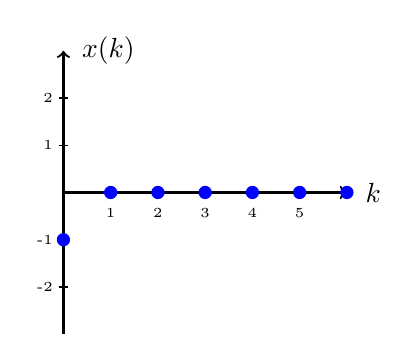
\begin{tikzpicture}[scale=0.6]
	\draw[thick][->](0,0)--(6,0) node [right=3pt]{$k$};
	\draw[thick][->](0,-3)--(0,3) node [right=3pt]{$x(k)$};

	\foreach \y [count=\i] in {-2,...,-1} {{
	     \draw (-0.1,\y) -- (0.1,\y) node [left=2pt]{{\tiny \y}};
 	}}
	\foreach \y [count=\i] in {1,...,2} {{
	     \draw (-0.1,\y) -- (0.1,\y) node [left=2pt]{{\tiny \y}};
 	}}
	\foreach \x [count=\i] in {-4,...,-1} {{
	    % \draw (\x,-0.1) -- (\x,0.1) node [below=4pt]{{\tiny \x}};
 	}}
	\foreach \x [count=\i] in {1,...,5} {{
	     \draw (\x,-0.1) -- (\x,0.1) node [below=4pt]{{\tiny \x}};
 	}}
		
	% koniec Osi
	
	\fill[fill=blue](0,-1) circle(4pt);
	\fill[fill=blue](1,0) circle(4pt);
	\fill[fill=blue](2,0) circle(4pt);
	\fill[fill=blue](3,0) circle(4pt);
	\fill[fill=blue](4,0) circle(4pt);
	\fill[fill=blue](5,0) circle(4pt);
	\fill[fill=blue](6,0) circle(4pt);
\end{tikzpicture}
\end{figure}

\pagebreak
%###################                 3.1.2              #################################%
\subsection*{Zadanie 3.1.2} {\color{darkgray}
	Narysować rozwiązanie równania różnicowego $x(k+1)=\lambda_ix(k)$\\
	 dla $i=1,2,3$ gdzie \\
	$\lambda_1 = -1, \lambda_2=-\frac{1}{2}, \lambda_3=1$ \\
	przy czym $x(0)=1$ i $k\geq0$
}\\\\
\noindent$\bullet\ \ \lambda_1 = -1$\\
$x(k+1)=-x(k)$\\
$x(k)=(-1)^k\cdot1=(-1)^k$

\begin{figure}[!h]
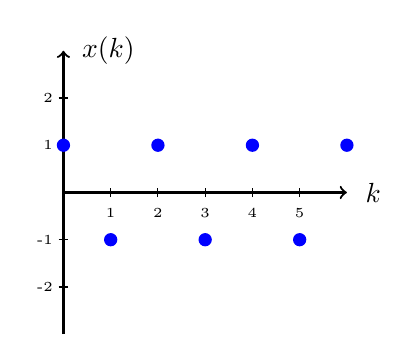
\begin{tikzpicture}[scale=0.6]
	\draw[thick][->](0,0)--(6,0) node [right=3pt]{$k$};
	\draw[thick][->](0,-3)--(0,3) node [right=3pt]{$x(k)$};

	\foreach \y [count=\i] in {-2,...,-1} {{
	     \draw (-0.1,\y) -- (0.1,\y) node [left=2pt]{{\tiny \y}};
 	}}
	\foreach \y [count=\i] in {1,...,2} {{
	     \draw (-0.1,\y) -- (0.1,\y) node [left=2pt]{{\tiny \y}};
 	}}
	\foreach \x [count=\i] in {-4,...,-1} {{
	    % \draw (\x,-0.1) -- (\x,0.1) node [below=4pt]{{\tiny \x}};
 	}}
	\foreach \x [count=\i] in {1,...,5} {{
	     \draw (\x,-0.1) -- (\x,0.1) node [below=4pt]{{\tiny \x}};
 	}}
		
	% koniec Osi
	
	\fill[fill=blue](0,1) circle(4pt);
	\fill[fill=blue](1,-1) circle(4pt);
	\fill[fill=blue](2,1) circle(4pt);
	\fill[fill=blue](3,-1) circle(4pt);
	\fill[fill=blue](4,1) circle(4pt);
	\fill[fill=blue](5,-1) circle(4pt);
	\fill[fill=blue](6,1) circle(4pt);
\end{tikzpicture}
\end{figure}


\noindent$\bullet\ \ \lambda_2 = -\frac{1}{2}$\\
$x(k+1)=-\frac{1}{2}\cdot x(k)$\\
$x(k)=(-\frac{1}{2})^k\cdot 1=(-\frac{1}{2})^k$

\begin{figure}[!h]
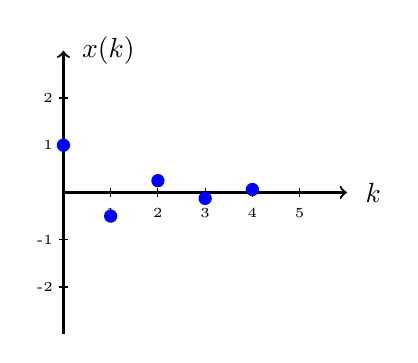
\begin{tikzpicture}[scale=0.6]
	\draw[thick][->](0,0)--(6,0) node [right=3pt]{$k$};
	\draw[thick][->](0,-3)--(0,3) node [right=3pt]{$x(k)$};

	\foreach \y [count=\i] in {-2,...,-1} {{
	     \draw (-0.1,\y) -- (0.1,\y) node [left=2pt]{{\tiny \y}};
 	}}
	\foreach \y [count=\i] in {1,...,2} {{
	     \draw (-0.1,\y) -- (0.1,\y) node [left=2pt]{{\tiny \y}};
 	}}
	\foreach \x [count=\i] in {-4,...,-1} {{
	    % \draw (\x,-0.1) -- (\x,0.1) node [below=4pt]{{\tiny \x}};
 	}}
	\foreach \x [count=\i] in {1,...,5} {{
	     \draw (\x,-0.1) -- (\x,0.1) node [below=4pt]{{\tiny \x}};
 	}}
		
	% koniec Osi
	
	\fill[fill=blue](0,1) circle(4pt);
	\fill[fill=blue](1,-0.5) circle(4pt);
	\fill[fill=blue](2,0.25) circle(4pt);
	\fill[fill=blue](3,-0.125) circle(4pt);
	\fill[fill=blue](4,0.0625) circle(4pt);
\end{tikzpicture}
\end{figure}

\noindent$\bullet\ \ \lambda_3 = 1$\\
$x(k+1)=x(k)$\\
$x(k)=1^k\cdot1 =1$

\begin{figure}[!h]
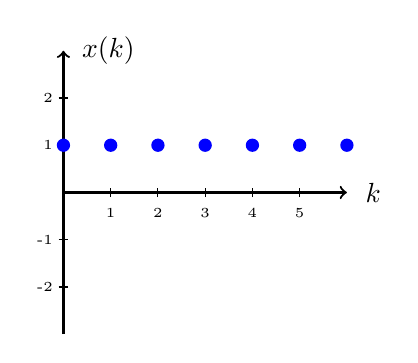
\begin{tikzpicture}[scale=0.6]
	\draw[thick][->](0,0)--(6,0) node [right=3pt]{$k$};
	\draw[thick][->](0,-3)--(0,3) node [right=3pt]{$x(k)$};

	\foreach \y [count=\i] in {-2,...,-1} {{
	     \draw (-0.1,\y) -- (0.1,\y) node [left=2pt]{{\tiny \y}};
 	}}
	\foreach \y [count=\i] in {1,...,2} {{
	     \draw (-0.1,\y) -- (0.1,\y) node [left=2pt]{{\tiny \y}};
 	}}
	\foreach \x [count=\i] in {-4,...,-1} {{
	    % \draw (\x,-0.1) -- (\x,0.1) node [below=4pt]{{\tiny \x}};
 	}}
	\foreach \x [count=\i] in {1,...,5} {{
	     \draw (\x,-0.1) -- (\x,0.1) node [below=4pt]{{\tiny \x}};
 	}}
		
	% koniec Osi
	
	\fill[fill=blue](0,1) circle(4pt);
	\fill[fill=blue](1,1) circle(4pt);
	\fill[fill=blue](2,1) circle(4pt);
	\fill[fill=blue](3,1) circle(4pt);
	\fill[fill=blue](4,1) circle(4pt);
	\fill[fill=blue](5,1) circle(4pt);
	\fill[fill=blue](6,1) circle(4pt);
\end{tikzpicture}
\end{figure}

\pagebreak
%###################                 3.1.3              #################################%
\subsection*{Zadanie 3.1.3} {\color{darkgray}
	Narysować rozwiązanie równania różnicowego $x(k+1)=\lambda_ix(k)$\\
	 dla $i=1,2,3$ gdzie \\
	$\lambda_1 = 0, \lambda_2=1, \lambda_3=-1$ \\
	przy czym $x(0)=1$ i $k\geq0$
}\\\\
\noindent$\bullet\ \lambda_1 = 0$\\

\begin{figure}[!h]
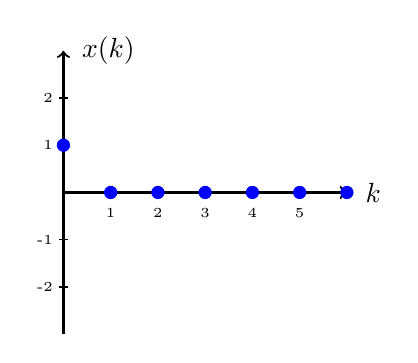
\begin{tikzpicture}[scale=0.6]
	\draw[thick][->](0,0)--(6,0) node [right=3pt]{$k$};
	\draw[thick][->](0,-3)--(0,3) node [right=3pt]{$x(k)$};

	\foreach \y [count=\i] in {-2,...,-1} {{
	     \draw (-0.1,\y) -- (0.1,\y) node [left=2pt]{{\tiny \y}};
 	}}
	\foreach \y [count=\i] in {1,...,2} {{
	     \draw (-0.1,\y) -- (0.1,\y) node [left=2pt]{{\tiny \y}};
 	}}
	\foreach \x [count=\i] in {-4,...,-1} {{
	    % \draw (\x,-0.1) -- (\x,0.1) node [below=4pt]{{\tiny \x}};
 	}}
	\foreach \x [count=\i] in {1,...,5} {{
	     \draw (\x,-0.1) -- (\x,0.1) node [below=4pt]{{\tiny \x}};
 	}}
		
	% koniec Osi
	
	\fill[fill=blue](0,1) circle(4pt);
	\fill[fill=blue](1,0) circle(4pt);
	\fill[fill=blue](2,0) circle(4pt);
	\fill[fill=blue](3,0) circle(4pt);
	\fill[fill=blue](4,0) circle(4pt);
	\fill[fill=blue](5,0) circle(4pt);
	\fill[fill=blue](6,0) circle(4pt);
\end{tikzpicture}
\end{figure}


\noindent$\bullet\ \lambda_2 = 1$\\

\begin{figure}[!h]
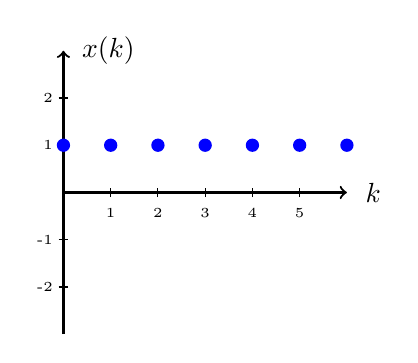
\begin{tikzpicture}[scale=0.6]
	\draw[thick][->](0,0)--(6,0) node [right=3pt]{$k$};
	\draw[thick][->](0,-3)--(0,3) node [right=3pt]{$x(k)$};

	\foreach \y [count=\i] in {-2,...,-1} {{
	     \draw (-0.1,\y) -- (0.1,\y) node [left=2pt]{{\tiny \y}};
 	}}
	\foreach \y [count=\i] in {1,...,2} {{
	     \draw (-0.1,\y) -- (0.1,\y) node [left=2pt]{{\tiny \y}};
 	}}
	\foreach \x [count=\i] in {-4,...,-1} {{
	    % \draw (\x,-0.1) -- (\x,0.1) node [below=4pt]{{\tiny \x}};
 	}}
	\foreach \x [count=\i] in {1,...,5} {{
	     \draw (\x,-0.1) -- (\x,0.1) node [below=4pt]{{\tiny \x}};
 	}}
		
	% koniec Osi
	
	\fill[fill=blue](0,1) circle(4pt);
	\fill[fill=blue](1,1) circle(4pt);
	\fill[fill=blue](2,1) circle(4pt);
	\fill[fill=blue](3,1) circle(4pt);
	\fill[fill=blue](4,1) circle(4pt);
	\fill[fill=blue](5,1) circle(4pt);
	\fill[fill=blue](6,1) circle(4pt);
\end{tikzpicture}
\end{figure}

\noindent$\bullet\ \lambda_3 = -1$\\

\begin{figure}[!h]
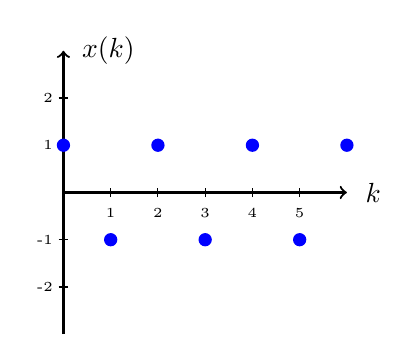
\begin{tikzpicture}[scale=0.6]
	\draw[thick][->](0,0)--(6,0) node [right=3pt]{$k$};
	\draw[thick][->](0,-3)--(0,3) node [right=3pt]{$x(k)$};

	\foreach \y [count=\i] in {-2,...,-1} {{
	     \draw (-0.1,\y) -- (0.1,\y) node [left=2pt]{{\tiny \y}};
 	}}
	\foreach \y [count=\i] in {1,...,2} {{
	     \draw (-0.1,\y) -- (0.1,\y) node [left=2pt]{{\tiny \y}};
 	}}
	\foreach \x [count=\i] in {-4,...,-1} {{
	    % \draw (\x,-0.1) -- (\x,0.1) node [below=4pt]{{\tiny \x}};
 	}}
	\foreach \x [count=\i] in {1,...,5} {{
	     \draw (\x,-0.1) -- (\x,0.1) node [below=4pt]{{\tiny \x}};
 	}}
		
	% koniec Osi

	\fill[fill=blue](0,1) circle(4pt);
	\fill[fill=blue](1,-1) circle(4pt);
	\fill[fill=blue](2,1) circle(4pt);
	\fill[fill=blue](3,-1) circle(4pt);
	\fill[fill=blue](4,1) circle(4pt);
	\fill[fill=blue](5,-1) circle(4pt);
	\fill[fill=blue](6,1) circle(4pt);
	
\end{tikzpicture}
\end{figure}
























\pagebreak
%###################                 3.2.1                #################################%
\subsection*{Zadanie 3.2.1} {\color{darkgray}
	Narysować rozwiązanie równania różnicowego $x(k+1)=x(k)+u_i(k)$\\
	dla $i=1,2,3$ gdzie \\
	$u_1 = -2, u_2=2,u_3=1$ \\
	przy czym $x(0)=0$ i $k\geq0$
}\\\\
$x(k+1)=Ax(i)+Bu(i)$\\
$x(k)=A^kx(0)+\sum^{k-1}_{j=0}A^{k-1-j}Bu(j)$\\
${\color{lightgray}A=1, B=1, \forall j \ \ \ u(j)=u_i }$\\
$\Rightarrow x(k)=x(0)+\sum^{k-1}_{j=0}u$ dla $x(0)=0$\\
$\Rightarrow x(k)=u_i\cdot k$\\

\noindent$\bullet\ \ i=1, u_i = -2$

\begin{figure}[!h]
\begin{tikzpicture}[scale=0.5]
	\draw[thick][->](0,0)--(6,0) node [right=3pt]{$k$};
	\draw[thick][->](0,-6)--(0,2) node [right=3pt]{$x(k)$};

	\foreach \y [count=\i] in {-5,...,-1} {{
	     \draw (-0.1,\y) -- (0.1,\y) node [left=2pt]{{\tiny \y}};
 	}}
	\foreach \y [count=\i] in {1,...,1} {{
	     \draw (-0.1,\y) -- (0.1,\y) node [left=2pt]{{\tiny \y}};
 	}}
	\foreach \x [count=\i] in {-4,...,-1} {{
	    % \draw (\x,-0.1) -- (\x,0.1) node [below=4pt]{{\tiny \x}};
 	}}
	\foreach \x [count=\i] in {1,...,5} {{
	     \draw (\x,-0.1) -- (\x,0.1) node [below=4pt]{{\tiny \x}};
 	}}
		
	% koniec Osi
	
	\fill[fill=blue](0,0) circle(4pt);
	\fill[fill=blue](1,-2) circle(4pt);
	\fill[fill=blue](2,-4) circle(4pt);
	\fill[fill=blue](3,-6) circle(4pt);
\end{tikzpicture}
\end{figure}

\noindent$\bullet\ \ i=2, u_i = 2$

\begin{figure}[!h]
\begin{tikzpicture}[scale=0.5]
	\draw[thick][->](0,0)--(6,0) node [right=3pt]{$k$};
	\draw[thick][->](0,-2)--(0,6) node [right=3pt]{$x(k)$};

	\foreach \y [count=\i] in {-1,...,-1} {{
	     \draw (-0.1,\y) -- (0.1,\y) node [left=2pt]{{\tiny \y}};
 	}}
	\foreach \y [count=\i] in {1,...,5} {{
	     \draw (-0.1,\y) -- (0.1,\y) node [left=2pt]{{\tiny \y}};
 	}}
	\foreach \x [count=\i] in {-4,...,-1} {{
	    % \draw (\x,-0.1) -- (\x,0.1) node [below=4pt]{{\tiny \x}};
 	}}
	\foreach \x [count=\i] in {1,...,5} {{
	     \draw (\x,-0.1) -- (\x,0.1) node [below=4pt]{{\tiny \x}};
 	}}
		
	% koniec Osi
	
	\fill[fill=blue](0,0) circle(4pt);
	\fill[fill=blue](1,2) circle(4pt);
	\fill[fill=blue](2,4) circle(4pt);
	\fill[fill=blue](3,6) circle(4pt);
\end{tikzpicture}
\end{figure}

\noindent$\bullet\ \  i=3, u_i = 1$

\begin{figure}[!h]
\begin{tikzpicture}[scale=0.5]
	\draw[thick][->](0,0)--(6,0) node [right=3pt]{$k$};
	\draw[thick][->](0,-2)--(0,6) node [right=3pt]{$x(k)$};

	\foreach \y [count=\i] in {-1,...,-1} {{
	     \draw (-0.1,\y) -- (0.1,\y) node [left=2pt]{{\tiny \y}};
 	}}
	\foreach \y [count=\i] in {1,...,5} {{
	     \draw (-0.1,\y) -- (0.1,\y) node [left=2pt]{{\tiny \y}};
 	}}
	\foreach \x [count=\i] in {-4,...,-1} {{
	    % \draw (\x,-0.1) -- (\x,0.1) node [below=4pt]{{\tiny \x}};
 	}}
	\foreach \x [count=\i] in {1,...,5} {{
	     \draw (\x,-0.1) -- (\x,0.1) node [below=4pt]{{\tiny \x}};
 	}}
		
	% koniec Osi
	
	\fill[fill=blue](0,0) circle(4pt);
	\fill[fill=blue](1,1) circle(4pt);
	\fill[fill=blue](2,2) circle(4pt);
	\fill[fill=blue](3,3) circle(4pt);
	\fill[fill=blue](4,4) circle(4pt);
	\fill[fill=blue](5,5) circle(4pt);
\end{tikzpicture}
\end{figure}

\pagebreak
%###################                 3.2.2                #################################%
\subsection*{Zadanie 3.2.2} {\color{darkgray}
	Narysować rozwiązanie równania różnicowego $x(k+1)=2x(k)+u_i(k)$\\
	dla $i=1,2,3$ gdzie \\
	$u_1 = 0, u_2=-2,u_3=2$ \\
	przy czym $x(0)=0$ i $k\geq0$
}\\\\
\noindent$\bullet\ \ u_1 = 0$\\
$x(k+1)=2x(k)+0$\\
$x(k)=2^k\cdot 0 = 0$

\begin{figure}[!h]
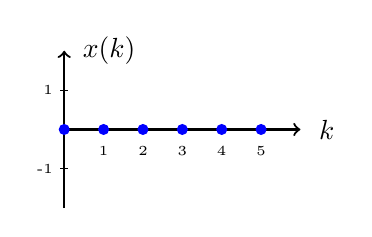
\begin{tikzpicture}[scale=0.5]
	\draw[thick][->](0,0)--(6,0) node [right=3pt]{$k$};
	\draw[thick][->](0,-2)--(0,2) node [right=3pt]{$x(k)$};

	\foreach \y [count=\i] in {-1,...,-1} {{
	     \draw (-0.1,\y) -- (0.1,\y) node [left=2pt]{{\tiny \y}};
 	}}
	\foreach \y [count=\i] in {1,...,1} {{
	     \draw (-0.1,\y) -- (0.1,\y) node [left=2pt]{{\tiny \y}};
 	}}
	\foreach \x [count=\i] in {-4,...,-1} {{
	    % \draw (\x,-0.1) -- (\x,0.1) node [below=4pt]{{\tiny \x}};
 	}}
	\foreach \x [count=\i] in {1,...,5} {{
	     \draw (\x,-0.1) -- (\x,0.1) node [below=4pt]{{\tiny \x}};
 	}}
		
	% koniec Osi
	
	\fill[fill=blue](0,0) circle(4pt);
	\fill[fill=blue](1,0) circle(4pt);
	\fill[fill=blue](2,0) circle(4pt);
	\fill[fill=blue](3,0) circle(4pt);
	\fill[fill=blue](4,0) circle(4pt);
	\fill[fill=blue](5,0) circle(4pt);
\end{tikzpicture}
\end{figure}

\noindent$\bullet\ \ u_2=-2$\\
$x(k+1)=2x(k)-2$\\
$x(k)=2^k \cdot 0 + \sum^{k-1}_{j=0}2^{k-1-j}\cdot(-2)=-2\cdot \sum^{k-1}_{j=0}(2^k\cdot 2^{-1}\cdot 2^{-j})$\\
$=-2^k\cdot \sum^{k-1}_{j=0}(\frac{1}{2})^j=-2^k\cdot\frac{1-(\frac{1}{2})^k}{1-\frac{1}{2}}=-2^{k+1}+2$

\begin{figure}[!h]
\begin{tikzpicture}[scale=0.5]
	\draw[thick][->](0,0)--(6,0) node [right=3pt]{$k$};
	\draw[thick][->](0,-7)--(0,2) node [right=3pt]{$x(k)$};

	\foreach \y [count=\i] in {-6,...,-1} {{
	     \draw (-0.1,\y) -- (0.1,\y) node [left=2pt]{{\tiny \y}};
 	}}
	\foreach \y [count=\i] in {1,...,1} {{
	     \draw (-0.1,\y) -- (0.1,\y) node [left=2pt]{{\tiny \y}};
 	}}
	\foreach \x [count=\i] in {-4,...,-1} {{
	    % \draw (\x,-0.1) -- (\x,0.1) node [below=4pt]{{\tiny \x}};
 	}}
	\foreach \x [count=\i] in {1,...,5} {{
	     \draw (\x,-0.1) -- (\x,0.1) node [below=4pt]{{\tiny \x}};
 	}}
		
	% koniec Osi
	
	\fill[fill=blue](0,0) circle(4pt);
	\fill[fill=blue](1,-2) circle(4pt);
	\fill[fill=blue](2,-6) circle(4pt);
\end{tikzpicture}
\end{figure}

\noindent$\bullet\ \ u_3=2$\\
$x(k+1)=2x(k)+2$\\
$x(k)=2^k \cdot 0 + \sum^{k-1}_{j=0}2^{k-1-j}\cdot(2)=2\cdot \sum^{k-1}_{j=0}(2^k\cdot 2^{-1}\cdot 2^{-j})$\\
$=2^k\cdot \sum^{k-1}_{j=0}(\frac{1}{2})^j=2^k\cdot\frac{1-(\frac{1}{2})^k}{1-\frac{1}{2}}=2^{k+1}-2$

\begin{figure}[!h]
\begin{tikzpicture}[scale=0.5]
	\draw[thick][->](0,0)--(6,0) node [right=3pt]{$k$};
	\draw[thick][->](0,-2)--(0,7) node [right=3pt]{$x(k)$};

	\foreach \y [count=\i] in {-1,...,-1} {{
	     \draw (-0.1,\y) -- (0.1,\y) node [left=2pt]{{\tiny \y}};
 	}}
	\foreach \y [count=\i] in {1,...,6} {{
	     \draw (-0.1,\y) -- (0.1,\y) node [left=2pt]{{\tiny \y}};
 	}}
	\foreach \x [count=\i] in {-4,...,-1} {{
	    % \draw (\x,-0.1) -- (\x,0.1) node [below=4pt]{{\tiny \x}};
 	}}
	\foreach \x [count=\i] in {1,...,5} {{
	     \draw (\x,-0.1) -- (\x,0.1) node [below=4pt]{{\tiny \x}};
 	}}
		
	% koniec Osi
	
	\fill[fill=blue](0,0) circle(4pt);
	\fill[fill=blue](1,2) circle(4pt);
	\fill[fill=blue](2,6) circle(4pt);
\end{tikzpicture}
\end{figure}




















\pagebreak
%###################                 3.3.1               #################################%
\subsection*{Zadanie 3.3.1} {\color{darkgray}
	Niech będzie dany układ ciągły opisany równaniem $\dot{x}(t)=ax(t)+bu(t)$\\
	(a) Znaleźć rozwiązanie tego układu dla: $x(0)=0, u(t)=1, a=-4, b=3$.\\
	(b) Znaleźć parametry układu dyskretnego, jeśli podł¡czono ekstrapolator pierwszego rzędu na wejściu
	i impulsator na wyjściu, przy czym pracuj¡ one synchronicznie z okresem próbkowania $t = 1$. 
	Rozwiązać powstały układ.\\
	(c) Jak wyżej, przy założeniu $t = 12$.\\
	(d) Narysować wszystkie rozwiązania na jednym układzie współrzędnych. Opisać różnice.\\
}\\\\
Brak rozwiązania


\pagebreak
%###################                 3.3.2               #################################%
\subsection*{Zadanie 3.3.2} {\color{darkgray}
	Niech będzie dany układ ciągły opisany równaniem $\dot{x}(t)=ax(t)+bu(t)$\\
	(a) Znaleźć rozwiązanie tego układu dla: $x(0)=0, u(t)=1, a=-1, b=2$.\\
	(b) Znaleźć parametry układu dyskretnego, jeśli podłączono ekstrapolator pierwszego rzędu na wejściu
	i impulsator na wyjściu, przy czym pracują one synchronicznie z okresem próbkowania $t = 1$. 
	Rozwiązać powstały układ.\\
	(c) Jak wyżej, przy założeniu $t = 10$.\\
	(d) Narysować wszystkie rozwiązania na jednym układzie współrzędnych. Opisać różnice.\\
}\\\\
(a)\\
$\dot{x}=-x+2$\\
$\frac{dx}{dt}=-x+2$\\
$\frac{dx}{-x+2}=dt$\\
$-\ln |-x+2|=t+c$, gdzie $c$ jest stałą \\
$\ln |-x+2|=-t+c$\\
$e^{-t+c}=-x+2$\\
$e^{-t}e^c=-x+2$\\
$ce^{-t}=-x+2$, bo $e^c$ to też stała\\

$x(0)=c+2=0 \Rightarrow c=-2$\\
$ce^{-t}=-x+2 \Rightarrow \boxed{x(t)=ce^{-t}+2=-2e^{-t}+2}$\\


\noindent
(b)\\
$h=1$\\
$x^+(i)=x(ih)=x(i)$\\
$u^+(i)=u(i)$\\
$y^+(i)=y(i)$\\
$A^+=e^{hA}=e^{-1}$\\
$B^+=\int_0^1e^{tA}B\ dt =\int_0^1e^{-t}2\ dt=2\int_0^1e^{-t}\ dt = -2e^t|^1_0=-2(e^{-1}-1)=2-\frac{2}{e}$\\
$C^+=C$\\
$x(i+1)=e^{-1}x(i)+(2-\frac{2}{e})u(i)=\frac{x(i)}{e}+2-\frac{2}{e}$\\
$x(k)=(e^{-1})^kx(0)+\sum_{j=0}^{k-1}(e^{-1})^{k-1-j}(2-\frac{2}{e})=(2-\frac{2}{e})\sum_{j=0}^{k-1}(e^{-k}\cdot e^1\cdot e^j)$\\
$=(2-\frac{2}{e})e^{1-k}\cdot\frac{1-e^k}{1-e}=2(e\cdot e^{-k} -e^{-k})\frac{1-e^k}{1-e}=2(-e^{-k})(1-e^k)=2-2e^{-k}$\\

\noindent
(c)\\
$h=10$\\
$x^+(i)=x(10i)$\\
$u^+(i)=u(10i)$\\
$A^+=e^{10A}=e^{-10}$\\
$B^+=2\int_0^{10}e^{-t} \ dt=2(-e^{-t}|_0^{10})=-2(e^{-10}-1)=2-2e^{-10}$\\
$x(k)=\underbrace{(e^{-10})^kx(0)}_{=0}+\sum_{j=0}^{k-1}(e^{-10})^{k-1-j}(2-2e^{-10})=(2-2e^{-10})\cdot e^{-10k-10}\cdot\frac{1-(e^{10})^k}{1-e^{10}}$\\
$=2(e^{-10k}\cdot e^{10}-e^{-10}\cdot e^{-10k}\cdot e^{10})\cdot\frac{1-e^{10k}}{1-e^{10}}=2(-e^{-10k}(1-e^{10}))\frac{1-e^{10k}}{1-e^{10}}=2-2e^{-10k}$\\

\begin{figure}[!h]
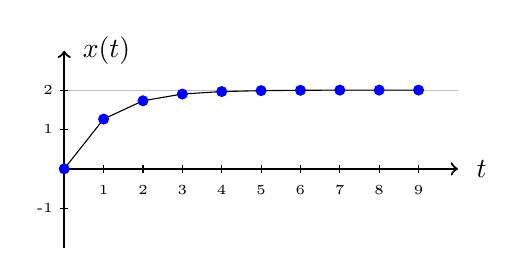
\begin{tikzpicture}[scale=0.5]
	\draw[draw=lightgray] (0,2) -- (10,2);
	\draw[thick][->](0,0)--(10,0) node [right=3pt]{$t$};
	\draw[thick][->](0,-2)--(0,3) node [right=3pt]{$x(t)$};

	\foreach \y [count=\i] in {-1,...,-1} {{
	     \draw (-0.1,\y) -- (0.1,\y) node [left=2pt]{{\tiny \y}};
 	}}
	\foreach \y [count=\i] in {1,...,2} {{
	     \draw (-0.1,\y) -- (0.1,\y) node [left=2pt]{{\tiny \y}};
 	}}
	\foreach \x [count=\i] in {1,...,9} {{
	     \draw (\x,-0.1) -- (\x,0.1) node [below=4pt]{{\tiny \x}};
 	}}
		
	% koniec Osi
	\draw (0,0)--(1,1.264)--(2,1.729)--(3,1.900)--(4,1.963)--(5,1.986)--(6,1.995)--(7,2)--(8,2) --(9,2);


	\fill[fill=blue](0,0) circle(4pt);
	\fill[fill=blue](1,1.264) circle(4pt);
	\fill[fill=blue](2,1.729) circle(4pt);
	\fill[fill=blue](3,1.900) circle(4pt);
	\fill[fill=blue](4,1.963) circle(4pt);
	\fill[fill=blue](5,1.986) circle(4pt);
	\fill[fill=blue](6,1.995) circle(4pt);
	\fill[fill=blue](7,2) circle(4pt);
	\fill[fill=blue](8,2) circle(4pt);
	\fill[fill=blue](9,2) circle(4pt);
\end{tikzpicture}
\end{figure}
- wykres (a) jest liniowy, (b) i (c) punktowe
- (a) punkty co 1, (b) punkty co 10 (?)




















\pagebreak
%###################                 3.4.1               #################################%
\subsection*{Zadanie 3.4.1} {\color{darkgray}
	Obliczyć $A^n$ dla macierzy\\
	$A=\left[ \begin{array}{cc} 4&-2\\0&2\end{array}\right]$
}\\\\
$A^n=PJP^{-1}$\\
$A^n=\underbrace{(PJP^{-1})(PJP^{-1})...(PJP^{-1})}_{n}$\\
$A^n=PJ^nP^{-1}$\\
$| [A-\lambda I] |=0$\\
$(4-\lambda)(2-\lambda)=0 \Rightarrow \lambda_1=4, \lambda_2=2$\\
$[A-\lambda I]\omega_1=0$\\
\\
$\left[ \begin{array}{cc}     0&-2\\0&-2    \end{array}\right]\left[ \begin{array}{c}     \omega_{11}\\\omega_{12}    \end{array}\right]=0
\ \ \ \ \ \begin{array}{c}    -2\omega_{12}=0 \\\omega_{11} \in \mathbb{R}    \end{array}
\ \ \ \ \ \omega_1=\left[ \begin{array}{c}     \omega_{11}\\0    \end{array}\right]=\left[ \begin{array}{c}     1\\0    \end{array}\right]$\\
\\\\
$\left[ \begin{array}{cc}     2&-2\\0&0    \end{array}\right]\left[ \begin{array}{c}     \omega_{21}\\\omega_{22}    \end{array}\right]=0
\ \ \ \ \ \begin{array}{c}    2\omega_{21}-2\omega_{22}=0 \\ \omega_{22}=\omega_{21}\\ \omega_{21} \in \mathbb{R}    \end{array}
\ \ \ \ \ \omega_2=\left[ \begin{array}{c}     \omega_{21}\\\omega_{21}    \end{array}\right]=\left[ \begin{array}{c}     1\\1 \end{array}\right]$\\
$P=[\omega_{1} \ \  \omega_{2}]=\left[ \begin{array}{cc}    1 &1\\0& 1   \end{array}\right]$\\
$P^{-1}=\frac{1}{det(P)}\left[ \begin{array}{cc}    1 &1\\0& 1   \end{array}\right]=\left[ \begin{array}{cc}    1 &-1\\0& 1   \end{array}\right]$\\
$J=\left[ \begin{array}{cc}     4&0\\0&2    \end{array}\right],J^n=\left[ \begin{array}{cc}     4^n&0\\0&2^n    \end{array}\right]$\\
$A^n=PJ^nP^{-1}=\left[ \begin{array}{cc}    1 &1\\0& 1   \end{array}\right]\left[ \begin{array}{cc}     4^n&0\\0&2^n    \end{array}\right]\left[ \begin{array}{cc}    1 &-1\\0& 1   \end{array}\right]=\left[ \begin{array}{cc}    4^n &2^n\\0& 2^n   \end{array}\right]\left[ \begin{array}{cc}    1 &-1\\0& 1   \end{array}\right]=\left[ \begin{array}{cc}    4^n &2^n-4^n\\0&2^n   \end{array}\right]$\\

\pagebreak
%###################                 3.4.2               #################################%
\subsection*{Zadanie 3.4.2} {\color{darkgray}
	Obliczyć $A^n$ dla macierzy\\
	$A=\left[ \begin{array}{cc} 2&1\\-4&0\end{array}\right]$
}\\\\
$A^n=PJ^nP^{-1}$\\
$| [A-\lambda I] |=(-\lambda)(2-\lambda)+4=\lambda^2-2\lambda+4=0$\\
$\Delta=4-16=-12$\\
$\lambda=1\pm i\sqrt{3}$\\
\\
$\boxed{\lambda=1+ i\sqrt{3}}$\\
\\
$[A-\lambda I]\omega_1=0$\\
\\
$\left[ \begin{array}{cc}     2-1-i\sqrt{3}&1\\-4&-1-i\sqrt{3}    \end{array}\right]\left[ \begin{array}{c}     \omega_{1}\\\omega_{2}    \end{array}\right]=\left[ \begin{array}{c}     0\\0    \end{array}\right]$\\
$\begin{array}{ll}    (1-i\sqrt{3})\omega_1+\omega_2=0 &\Rightarrow \omega_2=-(1-i\sqrt{3})\omega_1 \\ -4\omega_1+(-1-i\sqrt{3})\omega_2=0&\Rightarrow -4\omega_1+4\omega_1=0\end{array}$\\
$\ \ \ \ \ \omega=\left[ \begin{array}{c}     1\\-1+i\sqrt{3}    \end{array}\right]=\left[ \begin{array}{c}   1\\-1   \end{array}\right]+i\left[ \begin{array}{c}   0\\\sqrt{3}   \end{array}\right]$\\
\\\\
$P=\left[ \begin{array}{cc}    1&0\\-1&\sqrt{3}   \end{array}\right]$\\
$P^{-1}=\frac{1}{\sqrt{3}}\left[ \begin{array}{cc}    \sqrt{3}&0\\1&1   \end{array}\right]=\left[ \begin{array}{cc}   1&0\\ \frac{\sqrt{3}}{3}&\frac{\sqrt{3}}{3} \end{array}\right]$\\
\boxed{\begin{aligned}
	\lambda=a \pm ib\\
	tg \varphi=\frac{b}{a} \Rightarrow \varphi = arctg \frac{b}{a}\\
	J=\left[ \begin{array}{cc}     a&b\\-b&a    \end{array}\right] \rightarrow J^n=(\sqrt{a^2+b^2})^n \left[ \begin{array}{cc}     \cos n\varphi&\sin n \varphi\\-\sin n \varphi&\cos n \varphi    \end{array}\right]
\end{aligned}}\\
$\varphi=arctg \sqrt{3}=\frac{\pi}{3}$\\
$J^n=2^n\left[ \begin{array}{cc}     \cos n\frac{\pi}{3}&\sin n \frac{\pi}{3}\\-\sin n \frac{\pi}{3}&\cos n \frac{\pi}{3}    \end{array}\right]$\\
\\
$A^n=\left[ \begin{array}{cc}    1&0\\-1&\sqrt{3}   \end{array}\right]\cdot 2^n \cdot \left[ \begin{array}{cc}     \cos n\frac{\pi}{3}&\sin n \frac{\pi}{3}\\-\sin n \frac{\pi}{3}&\cos n \frac{\pi}{3}    \end{array}\right] \cdot \left[ \begin{array}{cc}   1&0\\ \frac{\sqrt{3}}{3}&\frac{\sqrt{3}}{3} \end{array}\right]$\\
$=2^n \left[ \begin{array}{cc}
	\cos+\frac{\sqrt{3}}{3}\sin   &  \frac{\sqrt{3}}{3} \sin \\
	-\frac{4}{3} \sqrt{3} \sin       &   -\frac{\sqrt{3}}{3} \sin + \cos
 \end{array}\right]$\\

\pagebreak
%###################                 3.4.3               #################################%
\subsection*{Zadanie 3.4.3} {\color{darkgray}
	Obliczyć $A^n$ dla macierzy\\
	$A=\left[ \begin{array}{cc} 3&-1\\-1&3\end{array}\right]$
}\\\\
$A^n=PJ^nP^{-1}$\\
$|A- \lambda I|=0$\\
$\left|\begin{array}{cc} 3-\lambda&-1\\-1&3-\lambda\end{array}\right|=(\lambda-3)^2-1=(\lambda-3-1)(\lambda-3+1)=(\lambda-4)(\lambda-2)=0$\\
$\begin{array}{cc}
\lambda_1=4 &\lambda_2=2\\
	(A-\lambda_1I)\omega_1=0		& (A-\lambda_1I)\omega_2=0 \\
	     \left[ \begin{array}{cc} -1&-1\\-1&-1\end{array}\right]  \left[ \begin{array}{c}\omega_{11}\\\omega_{12}\end{array}\right]
	&   \left[ \begin{array}{cc} 1&-1\\-1&1\end{array}\right]    \left[ \begin{array}{c}\omega_{21}\\\omega_{22}\end{array}\right]
	\\ -\omega_{11}-\omega_{12}=0	&\omega_{21}=\omega_{22}\\
	\omega_{12}=-\omega_{11}& \\
	\omega_1=\left[ \begin{array}{c}1\\-1\end{array}\right] 	&\omega_2=\left[ \begin{array}{c}1\\1\end{array}\right]
\end{array}$\\
${\color{lightgray}\boxed{      \frac{4^n}{2}=\frac{4^n}{4^\frac{1}{2}}=4^{n-\frac{1}{2}}=\frac{2^n}{2}=2^{n-1}      }}$\\
\\
$J=\left[ \begin{array}{cc}     4&0\\0&2    \end{array}\right]$\\
$J^n=\left[ \begin{array}{cc}     4^n&0\\0&2^n    \end{array}\right]$\\
$P=\left[ \begin{array}{cc}     1&1\\-1&1    \end{array}\right]$\\
$P^{-1}=\left[ \begin{array}{cc}     \frac{1}{2}&-\frac{1}{2}\\\frac{1}{2}&\frac{1}{2}    \end{array}\right]$\\
\\
$A^n=\left[ \begin{array}{cc}     1&1\\-1&1    \end{array}\right]
 \left[ \begin{array}{cc}     4^n&0\\0&2^n    \end{array}\right]
\left[ \begin{array}{cc}     \frac{1}{2}&-\frac{1}{2}\\\frac{1}{2}&\frac{1}{2}    \end{array}\right]
=
\left[ \begin{array}{cc}     4^n&2^n\\-4^n&2^n    \end{array}\right]
\left[ \begin{array}{cc}     \frac{1}{2}&-\frac{1}{2}\\\frac{1}{2}&\frac{1}{2}    \end{array}\right]
=
\left[ \begin{array}{cc}     
	4^{n-\frac{1}{2}}+2^{n-1}  &
	-4^{n-\frac{1}{2}}+2^{n-1} \\
	-4^{n-\frac{1}{2}}+2^{n-1} &
	4^{n-\frac{1}{2}}+2^{n-1}
\end{array}\right]
$\\















\pagebreak
%###################                 3.5.1               #################################%
\subsection*{Zadanie 3.5.1} {\color{darkgray}
	Do ciągłego systemu dynamicznego opisanego równaniami\\
	$\dot{x}_1(t)=2\pi x_2(t)$,\\
	$\dot{x}_2(t)=-2 \pi x_1(t)+u(t)$,\\
	podłączono ekstrapolator rzędu zerowego na wejściu i impulsator na wyjściu, przy czym pracują one synchronicznie z okresem próbkowania $h = 1 s$. Wyliczyć parametry systemu dyskretnego odpowiadające takiemu połączeniu.
}\\\\
$\dot{x}_1(t)=\left[ \begin{array}{cc}     0&2\pi\\-2\pi&0    \end{array}\right]_Ax(t)+\left[ \begin{array}{c}     0\\1    \end{array}\right]_Bu(t)$\\
$x^+(vi)=A^+x^+(i)+B^+u^+(i), h=1s$\\
$A^+=e^{hA}$\\
$A^+=e^{A}=Pe^JP^{-1}$\\
$\left[ \begin{array}{cc}     -\lambda&2\pi\\-2pi&-\lambda    \end{array}\right]=0 \Leftrightarrow \begin{array}{l}\lambda^2+4\pi^2=0 \\ \lambda=-4\pi^2 \\ \lambda_{1,2}=\pm 2\pi i\end{array} \begin{array}{l} \\ \\{\color{darkgray} (p=0, q=2\pi)} \end{array}$\\
$\left[ \begin{array}{cc}     -2\pi i& \boxed{2\pi } \\-2\pi&-2\pi i    \end{array}\right]
\left[ \begin{array}{c}   \omega_{11}  \\ \omega_{12}   \end{array}\right] =0$\\
$\begin{array}{r}\omega_{11} \in \mathbb{R}\\
-2\pi i \omega_{11}+2\pi \omega_{12}=0\\
\omega_{12}=i\omega_{11}\end{array} \Rightarrow \omega_1=\left[ \begin{array}{c}     \omega_{11}\\\omega_{12}    \end{array}\right]=
\omega_{11}\left[ \begin{array}{c}     1\\i    \end{array}\right]=
\omega_{11}\left[ \begin{array}{c}     1\\0    \end{array}\right]+ i\omega_{11}\left[ \begin{array}{c}     0\\1    \end{array}\right]$\\
$\Rightarrow P=\left[ \begin{array}{cc}     1&0\\0&1    \end{array}\right]=P^{-1}=I$\\
$\Rightarrow A$ jest postaci Jordana $\Rightarrow J=A=\left[ \begin{array}{cc}     0&2\pi\\-2\pi&0    \end{array}\right]$\\
$e^J=e^P \cdot\left[ \begin{array}{cc}     \cos(q)&\sin(q)\\-\sin(q)& \cos(q)   \end{array}\right]$\\
$e^J= \cdot\left[ \begin{array}{cc}     \cos(2\pi)&\sin(2\pi)\\-\sin(2\pi)& \cos(2\pi)   \end{array}\right]=\left[ \begin{array}{cc}     1&0\\0& 1   \end{array}\right]$\\
$Pe^JP^{-1}=\left[ \begin{array}{cc}     1&0\\0& 1   \end{array}\right]$\\
$B^+=\int^n_0e^{tA}B \ dt$\\
$B$ jest stałą\\
$B^+=\int^n_0e^{tA} \ dt \ B$\\
$\left| \begin{array}{c}tA=u-1\\t=uA \\dt=duA^{-1} \end{array}\right| B^+=\int_o^{hA}e^u\ du\ A^{-1}B=[e^{hA}-e^0]A^{-1}B$\\
$e^{hA}=e^A=\left[ \begin{array}{cc}     1&0\\0& 1   \end{array}\right]$\\
$e^0=1=J=\left[ \begin{array}{cc}     1&0\\0& 1   \end{array}\right]$\\
$\Rightarrow B^+=0=\left[ \begin{array}{c}    0\\0    \end{array}\right]$\\
$x^+(i+1)=A^+x^+(i)+B^+u^+(i)$\\
$x^+(i+1)=\left[ \begin{array}{cc}    1&0\\0&1    \end{array}\right]x^+(i)$\\


\pagebreak
%###################                 3.5.2               #################################%
\subsection*{Zadanie 3.5.2} {\color{darkgray}
	Do ciągłego systemu dynamicznego opisanego równaniami\\
	$\dot{x}(t)=Ax(t)+Bu(t)$,\\
	$y(t)=Cx(t)$,\\
	przy czym\\
	$A=\left[ \begin{array}{ccc}     -0.5&0&0\\0&-1&0\\0&0&-2    \end{array}\right], \ \ 
	B=\left[ \begin{array}{c}     1\\1\\1    \end{array}\right], \ \ 
	C=\left[ \begin{array}{ccc}     1&4&5\\3&1&9    \end{array}\right]$\\
	podłączono ekstrapolator rzędu zerowego na wejściu i impulsator na wyjściu, przy czym pracują one synchronicznie z okresem próbkowania $h = 1 s$. Wyliczyć parametry systemu dyskretnego odpowiadające takiemu połączeniu.
}\\\\
$x^+(i)=x(ih)=x(i)$\\
$y^+(i)=y(ih)=y(i)$\\
$u^+(i)=u(ih)=u(i)$\\
$A^+=e^{hA}$\\
A jest w postaci Jordana, więc $A=J$\\
$A^+=e^{hJ}=e^J=\left[ \begin{array}{ccc}     e^{-0.5}&0&0\\0&e^{-1}&0\\0&0&e^{-2}    \end{array}\right]$\\
$B^+=\int_0^he^{tA}B \ dt = \int_0^1\left[ \begin{array}{ccc}     e^{-0.5}&0&0\\0&e^{-1}&0\\0&0&e^{-2}    \end{array}\right]   
\left[ \begin{array}{c}     1\\1\\1    \end{array}\right] dt
= \int_0^1\left[ \begin{array}{c}   e^{-\frac{t}{2}} \\e^{-t} \\ e^{-2t}   \end{array}\right] dt$\\
$=\left[ \begin{array}{r}   -2e^{-\frac{t}{2}}|_0^1 \\-e^{-t}|_0^1 \\-\frac{1}{2} e^{-2t}|_0^1   \end{array}\right]
=\left[ \begin{array}{c}    2-2e^{-\frac{1}{2}}  \\  1-e^{-1} \\\frac{1}{2}-\frac{1}{2}e^{-2}  \end{array}\right]$\\
$C^+=C=\left[ \begin{array}{ccc}     1&4&5\\3&1&9    \end{array}\right]$\\


\pagebreak
%###################                 3.5.3               #################################%
\subsection*{Zadanie 3.5.3} {\color{darkgray}
	Do ciągłego systemu dynamicznego opisanego równaniami\\
	$\dot{x}_1(t)=-2x_1(t)+x_2(t)$,\\
	$\dot{x}_2(t)=-2x_1(t)$,\\
	podłączono ekstrapolator rzędu zerowego na wejściu i impulsator na wyjściu, przy czym pracują one synchronicznie z okresem próbkowania $h = 1 s$. Wyliczyć parametry systemu dyskretnego odpowiadające takiemu połączeniu.
}\\\\
$A=-2\ \ \ \ B=1\ \ \ \ \ C=-2$\\
$A^+=e^{Ah}=e^{-2}$\\
$B^+=\int_0^he^{tA}B\ dt=\int_0^he^{-2t}\ dt=|-\frac{1}{2}e^{-2t}|^h_0=-\frac{1}{2}e^{-2}$\\
$C^+=C=-2$\\
$\boxed{A^+=e^-2\ \ \ \ \ \ \ B^+=-\frac{1}{2}e^{-2}\ \ \ \ \ \ \ C^+=-2}$
































\pagebreak
%###################                 3.6.1               #################################%
\subsection*{Zadanie 3.6.1} {\color{darkgray}
	Dla jakich wartości parametrów $k_1$ i $k_2$ system dynamiczny\\
	$x(k+1)=\left[ \begin{array}{cc}     0&1\\-k_1&k_2    \end{array}\right]x(k)$\\
	będzie asymptotycznie stabilny. Zaznaczyć obszar stabilności na płaszczyźnie $k1 \times k2$
}\\\\
$x(k+1)=Ax(k)$\\
$| [A-\lambda I] | =0$\\
$(-\lambda)(k_2-\lambda)+k_1=0$\\
$\lambda^2-k_2\lambda+k_1=0$\\
$\lambda=\frac{z+1}{z-1}$\\
$(\frac{z+1}{z-1})^2-k_2(\frac{z+1}{z-1})+k_1=0$\\
$\frac{(z+1)^2-k_2(z+1)(z-1)+k_1(z-1)^2}{(z-1)^2}=0$\\
Rozważany układ jest asymptotycznie stabilny $\Leftrightarrow$ wartości własne ($\lambda$) macierzy $A$ leżą wewnątrz koła jednostkowego na płaszczyźnie zespolonej $\Leftrightarrow$ pierwiastki wielomianu $L(z)=(z+1)^2-k_2(z+1)(z-1)+k_1(z-1)^2$
leżą w lewej półpłaszczyźnie zespolonej $\Leftrightarrow$ spełnione jest dla wielomianu $L(z)$ kryterium Hurwitza\\
$L(z)=(z+1)^2-k_2(z+1)(z-1)+k_1(z-1)^2$\\
$L(z)=x^2+2z+1-k_2z^2+k_2+k_1z^2-2k_1z+k_1$\\
$L(z)=z^2(1+k_1-k_2)+z(2-2k_1)+(1+k_1+k_2)=0$\\
\\
W.K. $a_2>0, a_1>0, a_0>0$\\
\\
$\begin{array}{rl}    
	1+k_1-k_2&>0\\
	k_2&<k_1+1\\
	2-2k_1&>0\\
	k_1&<1\\
	1+k_1+k_2&>0\\
	k_2&>-k_1-1
\end{array}$\\
\\
$\left[ \begin{array}{cc}     a_1&0\\a_2&a_0    \end{array}\right]=
\left[ \begin{array}{cc}     2-2k_1&0\\1+k_1-k_2&1+k_1+k_2    \end{array}\right]$\\
$a_1>0 \wedge a_1a_0>0$ - spełnione dla W.K.\\
\begin{figure}[!h]
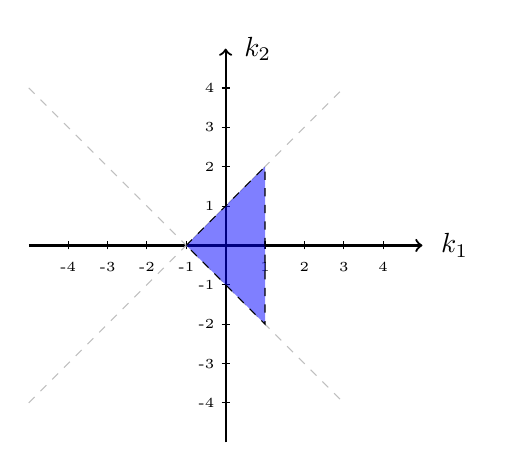
\begin{tikzpicture}[scale=0.5]
	\draw[thick][->](-5,0)--(5,0) node [right=3pt]{$k_1$};
	\draw[thick][->](0,-5)--(0,5) node [right=3pt]{$k_2$};

	\foreach \y [count=\i] in {-1,...,-4} {{
	     \draw (-0.1,\y) -- (0.1,\y) node [left=2pt]{{\tiny \y}};
 	}}
	\foreach \y [count=\i] in {1,...,4} {{
	     \draw (-0.1,\y) -- (0.1,\y) node [left=2pt]{{\tiny \y}};
 	}}
	\foreach \x [count=\i] in {-1,...,-4} {{
	     \draw (\x,-0.1) -- (\x,0.1) node [below=4pt]{{\tiny \x}};
 	}}
	\foreach \x [count=\i] in {1,...,4} {{
	     \draw (\x,-0.1) -- (\x,0.1) node [below=4pt]{{\tiny \x}};
 	}}
		
	% koniec Osi
	
	\draw[dashed, draw=lightgray] (-5,-4) -- (3,4);
	\draw[dashed, draw=lightgray] (-5,4) -- (3,-4);
	\draw[dashed, fill=blue,fill opacity=0.5] (-1,0)--(1,2)--(1,-2)--cycle;

	
\end{tikzpicture}
\end{figure}

\pagebreak
%###################                 3.6.2              #################################%
\subsection*{Zadanie 3.6.2} {\color{darkgray}
	Dla jakich wartości parametrów $k_1$ i $k_2$ system dynamiczny\\
	$x(k+1)=\left[ \begin{array}{ccc}    k_1-k_2 & 1 & 2 \\ 0 & k_1+k_2 & 1 \\ 0 & 0 & k_1^2+k_2^2    \end{array}\right]x(k)$\\
	będzie asymptotycznie stabilny. Zaznaczyć obszar stabilności na płaszczyźnie $k1 \times k2$
}\\\\
$\lambda_1 = k_1-k_2 \ \ \vee \  \ \lambda_2=k_1+k_2 \ \ \vee \ \ \lambda_3=k_1^2+k_2^2$\\
dyskretny system liniowy jesy asymprotycznie stabilny $\Leftrightarrow$ wartości własne macierzy $A$ leżą w kole jednostkowym o środku w zerze na płasczyźnie zespolonej (wystarczy sprawdzić warunek $|\lambda_i|<1$, nie trzeba z Hurwitza)\\
\\
$\bullet\ \ \lambda_1 = k_1-k_2 $\\
$\begin{array}{ccc}   k_1-k^2<1 & \wedge &k_1-k_2>-1 \\ k_2>k_1-1 & \wedge & k_2<k_1+1    \end{array}$\\
\\
$\bullet\ \ \lambda_1 =k_1+k_2$\\
$\begin{array}{ccc}  k_1+k_2<1 & \wedge & k_1+k_2>-1 \\ k_2<-k_1+1 & \wedge & k_2>-k_1-1    \end{array}$\\
\\
$\bullet\ \ \lambda_1 =k_1^2+k_2^2$\\
$\begin{array}{ccc}  k_1^2+k_2^2<1 &\wedge & k_1^2+k_2^2>-1  \end{array}$\\
\\
$\lambda_1 = k_1-k_2 \ \ \wedge \  \ \lambda_2=k_1+k_2 \ \ \wedge \ \ \lambda_3=k_1^2+k_2^2$\\

\begin{figure}[!h]
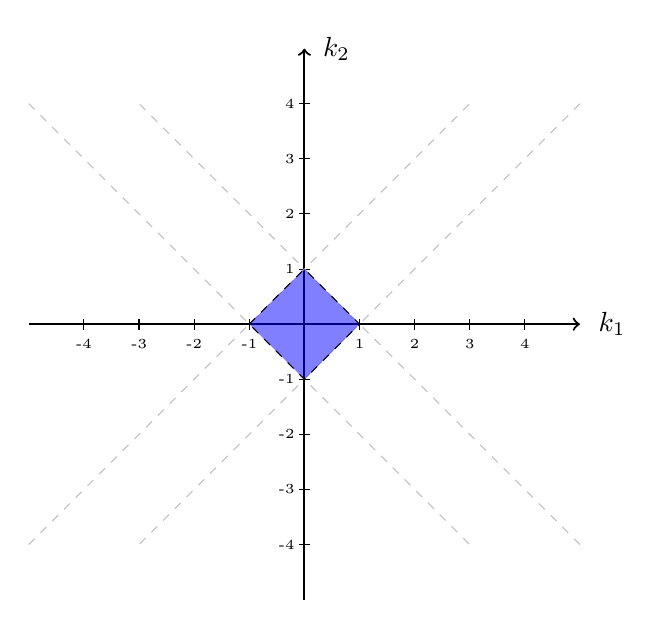
\begin{tikzpicture}[scale=0.7]
	\draw[thick][->](-5,0)--(5,0) node [right=3pt]{$k_1$};
	\draw[thick][->](0,-5)--(0,5) node [right=3pt]{$k_2$};

	\foreach \y [count=\i] in {-1,...,-4} {{
	     \draw (-0.1,\y) -- (0.1,\y) node [left=2pt]{{\tiny \y}};
 	}}
	\foreach \y [count=\i] in {1,...,4} {{
	     \draw (-0.1,\y) -- (0.1,\y) node [left=2pt]{{\tiny \y}};
 	}}
	\foreach \x [count=\i] in {-1,...,-4} {{
	     \draw (\x,-0.1) -- (\x,0.1) node [below=4pt]{{\tiny \x}};
 	}}
	\foreach \x [count=\i] in {1,...,4} {{
	     \draw (\x,-0.1) -- (\x,0.1) node [below=4pt]{{\tiny \x}};
 	}}
		
	% koniec Osi
	
	\draw[dashed, draw=lightgray] (-5,-4) -- (3,4);
	\draw[dashed, draw=lightgray] (-5,4) -- (3,-4);
	\draw[dashed, draw=lightgray] (5,-4) -- (-3,4);
	\draw[dashed, draw=lightgray] (5,4) -- (-3,-4);
	\draw[dashed, fill=blue,fill opacity=0.5] (-1,0)--(0,1)--(1,0)--(0,-1)--cycle;

	
\end{tikzpicture}
\end{figure}

\pagebreak
%###################                 3.6.3               #################################%
\subsection*{Zadanie 3.6.3} {\color{darkgray}
	Dla jakich wartości parametrów $k_1$ i $k_2$ system dynamiczny\\
	$x(k+1)=\left[ \begin{array}{cc}    -k_2&k_1\\-k_1&-k_2    \end{array}\right]x(k)$\\
	będzie asymptotycznie stabilny. Zaznaczyć obszar stabilności na płaszczyźnie $k1 \times k2$
}\\\\
$|A- \lambda I|=0$\\
$\left[ \begin{array}{cc}    -k_2-\lambda&k_1\\-k_1&-k_2-\lambda    \end{array}\right]=(k_2+\lambda)^2+k_1^2=(k_2+\lambda)^2-(ik_1)^2=(\lambda +k_2+ik_1)\cdot (\lambda+k_2-ik_1)=0$\\
\\
$\lambda=-k_2 \pm k_1$\\
Układ jest asymptotycznie stabilny, gdy wartości własne macierzy leżą wewnątrz koła jednostkowego na płaszczyźnie zespolonej o środku w zerze.\\
$|\lambda |<1$\\
$|\lambda|=\sqrt{(-k_2)^2+k_1^2}$\\
$\sqrt{k_1^2+k_2^2}<1$\\
$k_1^2+k_2^2<1$\\

\begin{figure}[!h]
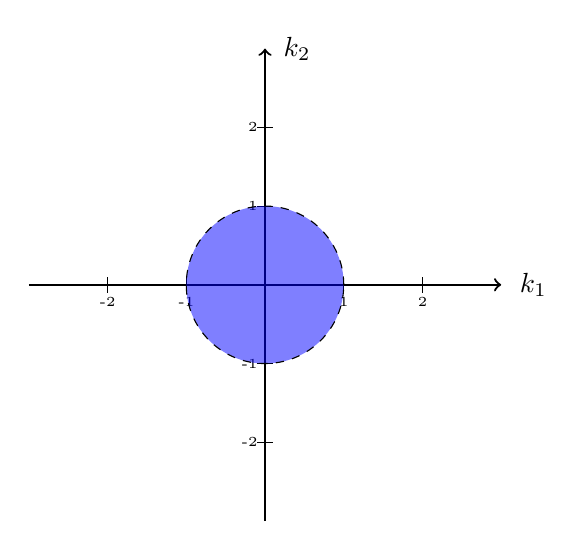
\begin{tikzpicture}
	\draw[thick][->](-3,0)--(3,0) node [right=3pt]{$k_1$};
	\draw[thick][->](0,-3)--(0,3) node [right=3pt]{$k_2$};

	\foreach \y [count=\i] in {-1,...,-2} {{
	     \draw (-0.1,\y) -- (0.1,\y) node [left=2pt]{{\tiny \y}};
 	}}
	\foreach \y [count=\i] in {1,...,2} {{
	     \draw (-0.1,\y) -- (0.1,\y) node [left=2pt]{{\tiny \y}};
 	}}
	\foreach \x [count=\i] in {-1,...,-2} {{
	     \draw (\x,-0.1) -- (\x,0.1) node [below=4pt]{{\tiny \x}};
 	}}
	\foreach \x [count=\i] in {1,...,2} {{
	     \draw (\x,-0.1) -- (\x,0.1) node [below=4pt]{{\tiny \x}};
 	}}
		
	% koniec Osi
	
	\draw[dashed, fill=blue,fill opacity=0.5] (0,0) circle (1);
\end{tikzpicture}
\end{figure}












\pagebreak
%###################                 3.7.1              #################################%
\subsection*{Zadanie 3.7.1} {\color{darkgray}
	Dla jakich wartości parametru $k_1$ system dynamiczny\\
	$x(k+1)=\left[ \begin{array}{cc}     -0.5k_1&0\\2&-k_1    \end{array}\right]x(k)$\\
	będzie niestabilny.
}\\\\
$(-0.5k_1-2)(-k_1-\lambda)=0$\\
$0.5k_1^2+0.5k_1\lambda+k_1\lambda+\lambda^2=0$\\
$\lambda^2+1.5k_1\lambda+0.5k_1^2=0$\\
$\lambda=\frac{z+1}{z-1}$\\
$(\frac{z+1}{z-1})^2-1.5k_1(\frac{z+1}{z-1})+0.5k_1^2=0$\\
$z^2+2z+1+1.5k_1z^2-1.5k_1+0.5k_1^2z^2-k_1^2z+0.5k_1^2=0$\\
$z^2\underbrace{(0.5k_1^2+1.5k_1+1)}_{a_2}+z\underbrace{(2-k_1^2)}_{a_1}+\underbrace{(0.5k_1^2-1.5k_1+1)}_{a_0}=0$\\\\
Z kryterium Hurwitza system będzie stabilny gdy:\\
 $\begin{array}{c}   a_2>0 \\ a_1>0 \\ a_0>0    \end{array} 
\Leftrightarrow  \begin{array}{r} 
	0.5k_1^2+1.5k_1+1>0 \\ 
	k_1^2+3k_1+2>0 \\
 	(k_1+1)(k_1+2)>0 
\end{array}   
\vee \begin{array}{r}
	2-k_1^2>0 \\
	(\sqrt{2}-k_1)(\sqrt{2}+k_1)>0\\
	(k_1-\sqrt{2})(\sqrt{2}+k_1)<0
\end{array}$
\begin{figure}[!h]
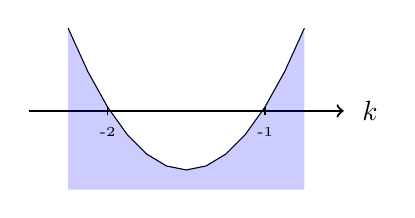
\begin{tikzpicture}[scale=0.5]
	\draw[thick][->](-4,0)--(4,0) node [right=3pt]{$k$};

	\draw(-3.0,2.1)--(-2.5,1.0)--(-2.0,0.1)--(-1.5,-0.6)--(-1.0,-1.1)--(-0.5,-1.4)
			--(0.0,-1.5)--(0.5,-1.4)--(1.0,-1.1)--(1.5,-0.6)--(2.0,0.1)--(2.5,1.0)--(3.0,2.1);
	\filldraw[draw opacity=0, fill=blue,fill opacity=0.2](-3.0,2.1)--(-2.5,1.0)--(-2.0,0.1)--(-1.5,-0.6)--(-1.0,-1.1)--(-0.5,-1.4)
			--(0.0,-1.5)--(0.5,-1.4)--(1.0,-1.1)--(1.5,-0.6)--(2.0,0.1)--(2.5,1.0)--(3.0,2.1)--(3,-2)--(-3,-2)--cycle;

	\draw (-2,-0.1) -- (-2,0.1) node [below=4pt]{{\tiny -2}};
	\draw (2,-0.1) -- (2,0.1) node [below=4pt]{{\tiny -1}};		
\end{tikzpicture}
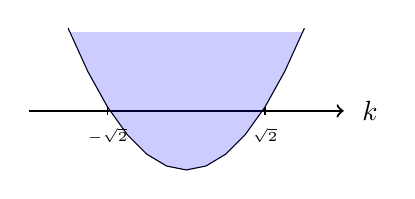
\begin{tikzpicture}[scale=0.5]
	\draw[thick][->](-4,0)--(4,0) node [right=3pt]{$k$};

	\draw(-3.0,2.1)--(-2.5,1.0)--(-2.0,0.1)--(-1.5,-0.6)--(-1.0,-1.1)--(-0.5,-1.4)
			--(0.0,-1.5)--(0.5,-1.4)--(1.0,-1.1)--(1.5,-0.6)--(2.0,0.1)--(2.5,1.0)--(3.0,2.1);
	\filldraw[draw opacity=0, fill=blue,fill opacity=0.2](-3.0,2.1)--(-2.5,1.0)--(-2.0,0.1)--(-1.5,-0.6)--(-1.0,-1.1)--(-0.5,-1.4)
			--(0.0,-1.5)--(0.5,-1.4)--(1.0,-1.1)--(1.5,-0.6)--(2.0,0.1)--(2.5,1.0)--(3.0,2.1)--(3,2)--(-3,2)--cycle;

	\draw (-2,-0.1) -- (-2,0.1) node [below=4pt]{{\tiny $-\sqrt{2}$}};
	\draw (2,-0.1) -- (2,0.1) node [below=4pt]{{\tiny $\sqrt{2}$}};		
\end{tikzpicture}
\end{figure}
ponieważ W.K. zawiera w sobie W.W., aby spełnione zostało kryterium Hurwitza musi być spełniony iloczyn warunków: $a_2>0 \wedge a_1>0$

\begin{figure}[!h]
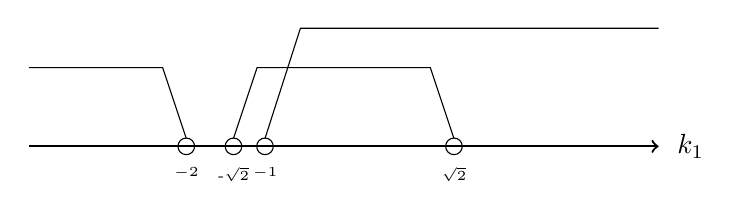
\begin{tikzpicture}
	\draw[thick][->](-4,0)--(4,0) node [right=3pt]{$k_1$};

	\draw(-4,1)--(-2.3,1)--(-2,0.1);
	\draw(-1.4,0.1)--(-1.1,1)--(1.1,1)--(1.4,0.1);
	\draw(-1,0.1)--(-0.55,1.5)--(4,1.5);

	\draw (-2,0) circle(3pt) node [below=4pt]{{\tiny $-2$}};
	\draw (-1.4,0) circle(3pt) node [below=4pt]{{\tiny -$\sqrt{2}$}};	
	\draw (-1,0) circle(3pt) node [below=4pt]{{\tiny $-1$}};	
	\draw (1.4,0) circle(3pt) node [below=4pt]{{\tiny $\sqrt{2}$}};
\end{tikzpicture}
\end{figure}
\noindent
$\Rightarrow$ układ jest stabilny $\Leftrightarrow k_1 \in (-1,\sqrt{2})$ \\
$\Rightarrow$ układ jest niestabilny $\Leftrightarrow k_1 \in (-\infty,-1) \cup (\sqrt{2},+\infty)$ \\

\pagebreak
%###################                 3.7.2              #################################%
\subsection*{Zadanie 3.7.2} {\color{darkgray}
	Dla jakich wartości parametru $k_1$ system dynamiczny\\
	$x(k+1)=\left[ \begin{array}{cc}    -1 &-k_1 \\ -k_1 &-3    \end{array}\right]x(k)$\\
	będzie niestabilny.
}\\\\
$\left| \begin{array}{cc}    -1 -\lambda&-k_1 \\ -k_1 &-3-\lambda    \end{array}\right|=(1+\lambda)(3+\lambda)-k_1^2=\lambda^2+3+4\lambda-k_1^2=0$\\
$\Delta=16-12+4k_1^2=4+4k_1^2$\\
$\lambda=-2 \pm \sqrt{1+k_1^2}$\\
\\
system będzie niestabilny $\Leftrightarrow |\lambda_i|>1$\\
\\
$\bullet\ \ \lambda=-2 + \sqrt{1+k_1^2}$\\
$ \begin{array}{ccc}
-2 + \sqrt{1+k_1^2}>1                &\vee&    -2 + \sqrt{1+k_1^2}<-1  \\
\sqrt{1+k_1^2}>3                           & &         \sqrt{1+k_1^2}<1 \\
k_1^2>8                                           & &                  k_1^2<0\\
k_1>2\sqrt{2} \vee k_1<-2\sqrt{2} & &                     \text{sprzeczne}\\
\end{array} $\\
\\\\
$\bullet\ \ \lambda=-2 - \sqrt{1+k_1^2}$\\
$ \begin{array}{ccc}
-2 - \sqrt{1+k_1^2}>1                &\vee&    -2 - \sqrt{1+k_1^2}<-1  \\
\sqrt{1+k_1^2}>-3                           & &         \sqrt{1+k_1^2}>-1 \\
\text{sprzeczne}                                & &                  k_1 \in \mathbb{R}
\end{array} $\\
\\\\
$\lambda=-2 + \sqrt{1+k_1^2} \vee \lambda=-2 - \sqrt{1+k_1^2} \Rightarrow k_1 \in \mathbb{R}$

\pagebreak
%###################                 3.7.3              #################################%
\subsection*{Zadanie 3.7.3} {\color{darkgray}
	Dla jakich wartości parametru $k_1$ system dynamiczny\\
	$x(k+1)=\left[ \begin{array}{cc}    -k_1 &k_1 \\ -k_1 &-k_1    \end{array}\right]x(k)$\\
	będzie niestabilny.
}\\\\
$\left[ \begin{array}{cc}    -k_1 -\lambda&k_1 \\ -k_1 &-k_1-\lambda    \end{array}\right]
=(-k_1-\lambda)^2+k_1^2=(-k_1-\lambda)^2-(ik_1)^2=(-k_1-\lambda-ik_1)(-k_1-\lambda+ik_1)=(\lambda+k_1-ik_1)(\lambda+k_1+ik_1)=0$\\
$\lambda=-k_1 \pm ik_1$\\
układ jest niestabilny gdy $|\lambda|>1$\\
podstawiamy tu moduł - więc usuwamy i z zespolonej.\\
$|\lambda|=\sqrt{(-k_1)^2+(k_1)^2}=\sqrt{k_1^2+k_1^2}>1$\\
$2k_1^2>1$\\
$k_1^2>\frac{1}{2}$\\
$k_1>\frac{\sqrt{2}}{2}$\\













\pagebreak
%###################                 3.8.1              #################################%
\subsection*{Zadanie 3.8.1} {\color{darkgray}
	Wyznaczyć rozwiązanie następującego równania różnicowego (rekurencyjnego)\\
	$x(k+2)+x(k+1)-2x(k)=0, x(0)=1,x(1)=-1$
}\\\\
zakładam rozwiązanie postaci $z^n$\\
$x^n, +z^{n-1}+2z^{n-2}=0$\\
$z^2+z-2=0$ - wielomian charakterystyczny\\
$W(z)=(z+2)(z-1)$\\
$z_1=-2, \ \ z_2=1$\\
rozwiązanie równania jest postaci:\\
$x(k)=Cz_1^k+Dz_2^k$\\
podstawiając $x(0)$ oraz $x(1)$\\
$\begin{cases} 
	x(0)=1=C+D \\
	x(1)=-1=Cz_1+Dz_2
\end{cases}$\\
$\begin{cases}
	 C=1-D \\
	-1=-2C+D
\end{cases}$\\
$\begin{cases}
	 D=1-C\\
	-1=-2C+1-C
\end{cases}$\\
$\begin{cases}
	 D=1-C\\
	3C=2
\end{cases}$\\
$C=\frac{2}{3} \ \ \ D=\frac{1}{3}$\\
$\Rightarrow x(k)=\frac{1}{3}(2 \cdot(-2)^k+1^k)$\\
$\boxed{x(k)=\frac{2}{3}(-2)^k+\frac{1}{3}1^k}$

\pagebreak
%###################                 3.8.2              #################################%
\subsection*{Zadanie 3.8.2} {\color{darkgray}
	Wyznaczyć rozwiązanie następującego równania różnicowego (rekurencyjnego)\\
	$x(k+2)+3x(k+1)+2x(k)=0, x(0)=2,x(1)=-3$
}\\\\
$q^{k+2}+3q^{k+1}+2q=0$\\
$q^2+3q+2=0$\\
$\Delta=9-8=1$\\
$q=\frac{-3+1}{2}=-1 \ \ \vee \ \ q=\frac{-3-1}{2}=-2$\\
$x(k)=a(-1)^k+b(-2)^k$\\
$\begin{cases} x(0)=a+b=2 \\ x(1)=-a-2b=-3\end{cases}$\\
$b=1 \wedge a=1$\\
$\boxed{x(k)=(-1)^k+(-2)^k}$

\pagebreak
%###################                 3.8.3              #################################%
\subsection*{Zadanie 3.8.3} {\color{darkgray}
	Wyznaczyć rozwiązanie następującego równania różnicowego (rekurencyjnego)\\
	$x(k+2)+2x(k+1)-3x(k)=0, x(0)=2,x(1)=-2$
}\\\\
$x^2+2x-3=0$\\
$\Delta=4+12=16, \sqrt{\Delta}=4$\\
$x_1=\frac{-2-4}{2}=-3 \wedge x_2=1$\\
$x(k)=C_1x_1^k+C_2x_2^k$\\
$\begin{cases} x(0)=2=C_1+C_2 \Rightarrow C_2=2-C_1 \\ x(1)=-2=-3C_1+C_2\end{cases}$\\
$-2=-3C_1+2-C_1 \Rightarrow C_1=1$\\
$C_2=1$\\
$\boxed{x(k)=-3^k+1}$\\

\noindent{\color{red}Alternatywne : }
\\
równanie charakterystyczne\\
$r^2+2r-3=0$\\
$(r+1)^2-4=0$\\
$(r+1-2)(r+1+2)=0$\\
$(r-1)(r+3)$\\
$r_1=1\ \ \ \ \ r_2=-3$\\
\\
$x(k)=c_1r_1^k+c_2r_2^k$\\
$x(0)=2=c_1+c_2$\\
$x(1)=-2=c_1+3c_2$\\
\\
$\begin{cases}2=c_1+c_2\\-2=c_1-3c_2 \end{cases}$\\
$4=4c_2$\\
$c_1=1\ \ \ \ c_2=1$\\
\\
$\boxed{x(k)=1+(-3)^k}$










\pagebreak
%###################                 3.9.1              #################################%
\subsection*{Zadanie 3.9.1} {\color{darkgray}
	Dany jest układ dyskretny\\
	$x(k+1)=Ax(k), A=\left[ \begin{array}{ccccc}    0&\cdots&0&0&0 \\  1&\cdots&0&0&0 \\\vdots&\ddots&\vdots&\vdots&\vdots \\ 1&\cdots&1&0&0    \\1&\cdots&1&1&0\end{array}\right]_{n \times n}$\\
	przy czym $k=1,2,...$ Wyznaczyć $x(n)$.
}\\\\
wielomian charakterystyczny: $| [A-\lambda I] |=0$\\
$\left[ \begin{array}{ccccc}    -\lambda&\cdots&0&0&0 \\  1&\cdots&0&0&0 \\\vdots&\ddots&\vdots&\vdots&\vdots \\ 1&\cdots&1&-\lambda&0    \\1&\cdots&1&1&-\lambda\end{array}\right]=(-\lambda)^n${\color{lightgray} (wyznacznik macierzy diagonalnej)}\\\\
Z Tw. Cagleya-Hamiltona wiadomo, że każda macierz spełnia swój wielomian charakterystyczny\\
$A^n=0 $\\\\
rozwiązanie równania $x(k+1)=Ax(k)$ ma postać $x(k)=A^kx(0)$ czyli $x(n)=A^nx(0)=0$\\
Biorąc więc pod uwagę fakt $A^n=0 $ wiadomo, że rozwiązanie x(k) stanie się zerem w cco najwyżej n krokach, niezależnie od warunku początkowego $x(0)$

\pagebreak
%###################                 3.9.2              #################################%
\subsection*{Zadanie 3.9.2} {\color{darkgray}
	Dany jest układ dyskretny\\
	$x(k+1)=Ax(k)+Bu(k), A=\left[ \begin{array}{ccccc}   
		 0&1&2&\cdots&n-1 \\
		 0&0&1&\cdots&n-2  \\
		 \vdots&\vdots&\vdots&\ddots&\vdots  \\
		 0&0&0&\cdots&1  \\
		 0&0&0&\cdots&0  \\
	\end{array}\right]_{n \times n}, \ \ \ \ B=\left[\begin{array}{c}   
		1 \\ 0 \\ \vdots \\ 0 \\ 0
	\end{array}\right]$\\
	przy czym $k=1,2,...$ Wyznaczyć $x(n)$ wiedząc, że $u(i)=1$ dla $i=1,2,...,n$.
}\\\\
$x(n)=A^nx(0)+\sum_{j=0}^{n-1}A^{n-1-j}Bu(j)$\\
Zauważmy, że $\det (A) = 0$ (bo same zera na przekątnej)\\
wtedy $\det(\lambda I-A)=\lambda^n$\\
z Tw. Cagleya-Hamiltona $A^n=0$ (każda macierz spełnia swój wielomian charakterystyczny)\\
mamy więc $A^nx(0)=0$, czyli $x(n)=\sum_{j=0}^{n-1}A^{n-1-j}B\underbrace{u(j)}_{=1}$\\
Przy kolejnych mnożeniach macierzy $A$ podniesionej do jakiejś potęgi przez $B$ otrzymujemy pierwszą kolumnę macierzy $A$, która zawiera same zera, poza przypadkiem $A^0=I$ (macierz jednostkowa), więc sumujemy $n-1$ kolumn samych zer oraz jedną równą $B \  (I\cdot B=B)$\\
ostatecznie $\boxed{x(n)=B}$

\pagebreak
%###################                 3.9.3              #################################%
\subsection*{Zadanie 3.9.3} {\color{darkgray}
	Dany jest układ dyskretny\\
	$x(k+1)=Ax(k)+Bu(k), A=\left[ \begin{array}{ccccc}   
		 0&1&1&\cdots&1 \\
		 0&0&1&\cdots&1  \\
		 \vdots&\vdots&\vdots&\ddots&\vdots  \\
		 0&0&0&\cdots&1  \\
		 0&0&0&\cdots&0  \\
	\end{array}\right]_{n \times n}, \ \ \ \ B=\left[\begin{array}{c}   
		1 \\ 0 \\ \vdots \\ 0 \\ 0
	\end{array}\right]$\\
	przy czym $k=1,2,...$ Wyznaczyć $x(n)$ wiedząc, że $u(i)=1$ dla $i=1,2,...,n$.
}\\\\
$|A|=0$\\
$x(k+1)=Ax(k)$\\
$|\lambda I -A|=\lambda^n$\\
z Tw. Cagleya-Hamiltona:\\
$A^n=0$\\
$x(1)=Ax(0)+B$\\
$x(2)=A^2x(0)+(A+1)B$\\
$x(3)=A^3x(0)+(A^2+A+1)B$\\
$...$\\
$x(n)=A^nx(0)+(A^{n-1}+A^{n-2}+...+1)B$\\
ponieważ tylko $A^n=0$, więc dla każdego $A^{n-1}, A^{n-2},...\neq0$\\
te potęgi będą miały jakieś śmieci w wartościach, nie istotne co tam będzie. Ważne, że tam gdzie w $A$ są $0$ nie pojawi się nic nowego, czyli gdzie było $0$ przed potęgowaniem, tam będzie też po. $\Rightarrow$ wynik iloczynu $A^iB=0$ (macierz zerowa), $i=1,...,n-1 \ \ \Rightarrow \boxed{x(n)=B}$ 

\pagebreak
%###################                 3.9.4              #################################%
\subsection*{Zadanie 3.9.4} {\color{darkgray}
	Dany jest układ dyskretny\\
	$x(k+1)=Ax(k), A=\left[ \begin{array}{ccccc}   
		 0&1&1&\cdots&1 \\
		 0&0&1&\cdots&1  \\
		 \vdots&\vdots&\vdots&\ddots&\vdots  \\
		 0&0&0&\cdots&1  \\
		 0&0&0&\cdots&0  \\
	\end{array}\right]_{n \times n}$\\
	przy czym $k=1,2,...$ Wyznaczyć $x(2n)$.
}\\\\
$|A|=0$\\
$x(k+1)=Ax(k)$\\
$|\lambda I -A|=\lambda^n$\\
z Tw. Cagleya-Hamiltona:\\
$A^n=0$\\
$x(1)=Ax(0)$\\
$x(2)=A^2x(0)$\\
$x(3)=A^3x(0)$\\
$...$\\
$x(n)=A^nx(0)=0$\\
$x(2n)=A^nx(n)=0$\\